
\section{绪论/Introduction}

\subsection{集成感知与通信（ISAC）基本介绍}

下一代无线网络（如超越5G（B5G）和6G）被视为推动众多新兴应用发展的关键基础设施。这些应用不仅需要高质量的无线连接，还对高精度、高鲁棒性的环境感知能力提出了更高要求。在关于B5G/6G网络的诸多前瞻性愿景中，一个普遍共识是：感知将在未来无线网络中发挥比以往更加重要的作用。

\begin{figure}[htbp]
	\centering
	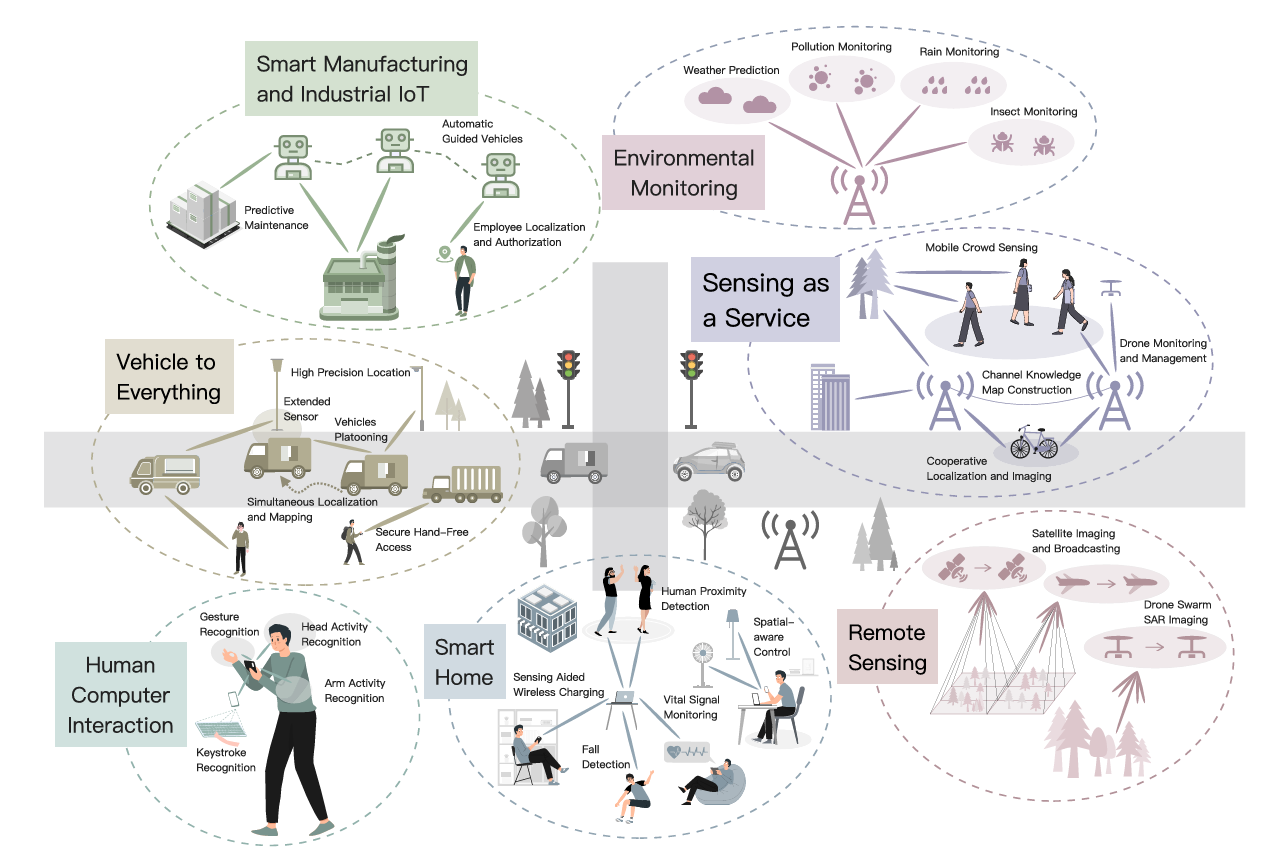
\includegraphics[width=0.8\textwidth]{img/1-1.png} % 图片文件名，不需要加扩展名
	\caption{用于未来无线网络的ISAC技术 \cite{9737357}}
	\label{fig:example}
\end{figure}


尽管针对未来无线系统的研究仍处于起步阶段，但当前技术发展趋势已清晰表明，我们正逐步具备在B5G和6G时代实现新型感知功能的技术基础。事实上，无线电感知与通信（Sensing and Communication，S\&C）系统均朝着更高频段、更大规模天线阵列以及设备小型化的方向发展，因此二者在硬件架构、信道特性以及信号处理等方面呈现出越来越高的相似性。这为利用现有无线基础设施实现感知功能创造了前所未有的机遇。

未来无线网络将突破传统通信服务的范畴，进一步提供无处不在的感知服务，实现对周围环境的测量甚至成像。网络所具备的感知能力及其获取环境感知数据的能力，被认为是未来智能世界实现环境认知、知识学习与智能构建的重要基础，并将在众多位置感知和环境感知场景中发挥关键作用。例如，车联网、智能家居、智能制造、遥感监测、环境监测以及人机交互等典型应用场景，如图1所示，相关内容将在第五节A部分进行详细介绍。

基于上述需求，迫切需要对B5G/6G网络中的感知与通信操作进行协同设计与联合优化，这也推动了近年来集成感知与通信（Integrated Sensing and Communication，ISAC）研究方向的迅速兴起。

\subsection{采用集成感知与通信技术的优点}

感知与通信的信息处理方式截然不同。感知负责从噪声观测中收集和提取信息，而通信则侧重于通过专门定制的信号传输信息，然后再从噪声环境中恢复信息。

ISAC的最终目标是将这两种操作统一起来，并在二者之间寻求直接的权衡以及相互提升的性能。一方面，ISAC 有望显著提高频谱效率和能量效率，同时降低硬件和信号传输成本，因为它试图将感知和通信融合到一个单一的系统中，而此前这两者需要争夺各种资源。另一方面，ISAC 还追求更深层次的融合，不再将这两种功能视为独立的最终目标，而是协同设计以实现互利共赢，例如通过通信辅助感知和感知辅助通信。



%\pagebreak


